\documentclass[12pt]{extarticle}

\usepackage{mathptmx,helvet,courier,bm}
\usepackage{amsmath,amssymb,stmaryrd}
\usepackage[sort&compress,numbers]{natbib}
\usepackage{url}
\usepackage{graphicx}
\usepackage{longtable}
\usepackage{fullpage}
\usepackage{setspace}
\usepackage{caption}
\usepackage{subcaption}



\setcounter{bottomnumber}{2}

% Personal commands
%
\newcommand{\equationname}{equation}

% Demarcate figures
\newcommand{\topfigrule}{\relax\noindent\rule[-6pt]{\columnwidth}{.4pt}}
\newcommand{\botfigrule}{\relax\noindent\rule[16pt]{\columnwidth}{.4pt}}

%
% A more standardized way of making paper titles
%
\author{Jacob Calder\footnote{jcalder@utexas.edu}, Iwo Dubaniowski \footnote{mduban@gmail.com}, C. Vic Hu \footnote{vic@cvhu.org}, Subhashini Venugopalan\footnote{vsubhashini@utexas.edu}\\[4pt]
\-\\
EE380L Data Mining\\
University of Texas at Austin\\
\url{https://github.com/cvhu/ee380l-ghosh-project}
}
\title{Mining for Spillovers in Patents}

\begin{document}
\sloppy

\maketitle
%\doublespace
\onehalfspace

\begin{center}
\textbf{Abstract}
\end{center}
This research sought to analyze the patent data to track knowledge spillovers (one innovation leading to another) in the field of solar innovation. Through the use of the topic modeling toolkit in the MAchine Learning for Language Toolkit (MALLET), the patent text was placed into topics and mapped into real world categories. Once we found the hidden thematic structure of the patent data, we were able to correlate the topic models to other meta-data such as technology area, CPC Class, year and geographical location, and inferred relevant knowledge spillovers accordingly.

\section{Introduction}
The project proposed by Professor Rai involves analyzing a set of approximately 1,000 patents that pertain to solar energy technologies obtained from the US Patent and Trademark Office\cite{us_patent}. The information provided for each patent contains the following attributes:

\begin{enumerate}
\item inventor(s)
\item assignees
\item dates of filing, application, and issue
\item keywords based on standard patent classifications
\item geographical location of the assignee firm or inventor
\end{enumerate}
 The patents have been pre-classified based on the portion of the supply chain to which the patents apply. Additionally, a large amount of preprocessing and web crawling for corrected information was done in order to insure a reliable data source.

The overall goal of the project is to develop a method of clustering the patents that will allow for the discovery of temporal and spatial connections between groups of patents linked to spillovers in innovation. In other words, it is not uncommon for an innovation to lead to other innovations. While this is intuitively easy to understand, it is not a trivial task to quantitatively track or measure. Traditionally, knowledge spillovers in patents is studied using citation linkages. However, this is not a reliable method; intellectual property attorneys often cite a wide variety of other patents to increase the chance of acceptance, which doesn't necessarily reflect the true relationships between innovations. We propose an alternative method to run a topic modeling algorithm over the abstract and claims texts of the patents. The patents are then sorted by the geographical location and the publishing date in the attempt to illustrate trends within certain topics.

\subsection{Motivation}
There is a significant amount of similar works performed in the area of copyright protection and IP portfolios management, including textual data mining such as key phrase extraction algorithms and co-word analysis in the context of patents \cite{TLY07}. Furthermore, there are works available on evaluating these methods to best fit the problem at hand \cite{TLY03}. Moreover, the idea of textual patents similarity is a subject of an ongoing research applicable to the cognitive science and legal (patents infringements) fields, resulting in different concepts of similarity measurements and coefficients \cite{MM10}.

By using a bag-of-words model such as topic modeling, it is interesting to analyze text-based hidden thematic structures between correlated patent publications. Our hypothesis assumes some underlying linguistic patterns introduced by knowledge spillover that aren't necessarily apparent in the context of citations. Although it is difficult to define and quantify such relations, we can reasonably verify our results with domain knowledges and geographical information \cite{geography}.

\subsection{Hypothesis}
By using latent Dirichlet allocation (LDA), the simplest topic modeling algorithm, we make the following assumptions about our patent documents:

\begin{itemize}
\item words have no dependencies with respect to their surrounding neighbors
\item document ordering is irrelevant
\item the number of topic is fixed and has to be determined manually
\end{itemize}

Although these assumptions made by LDA aren't necessarily ideal and realistic to capturing the complete syntactic information, they are simple and efficient enough to help us model the hidden topics and thus infer our spillover assumptions.

\section{Data}
 The data for this project was initially a database of approximately 1,000 entries containing 43 fields, including several forms of identification, classification, authors, owners, filing dates, and filing locations. The final analysis would use only 7 fields: patent number, filing year, city, state, country, tech area and CPC class. Additionally, the abstract and claims of the patent were added to the database after being scraped from the USPTO website.

\subsection{Source}
The database was assembled by a team working on the project for Professor Rai. The team manually read every patent that was returned when querying the patent office for a certain tech area. They then decided whether or not the patents were appropriate to the topic of this research. The team placed appropriate patents into tech areas based on their personal interpretation of the subject of the patent. Following this placement the patents were manually entered into the database along with all fields the team deemed important.

\subsection{Preprocessing}
Due to the hand-entered nature of the database, a fair portion of preprocessing was required. Firstly, many of the fields needed for the analysis contained inconsistently-formatted data. For example, many geographic locations would be surrounded by parentheses, have word orders switched, or have stray blank space that imposed difficulties in our analysis. To overcome this problem, the database ran through several preprocessing scripts to remove these abnormalities. An additional script was used to add more granularity to the geographic location, sorted by cities for California, by states for the rest of the United States, and by country for the rest of the world.

The next issue with data normalization was the corrupted data. On one hand, human-generated data is prone to erroneous results. On the other hand, most of the links provided by Dr. Rai's team have expired and no longer reflects the true intended data source (an updated version was provided later on). In an effort to overcome these problems, we wrote a web crawler to scrape relevant data directly from the USPTO website and recreated a cleaner and more consistent database.

\subsection{Challenges}

The primary challenges encountered were the previously mentioned hand-entered nature of the data and the poorly-formatted HTMLs on the USPTO website. A significant amount of time was dedicated to preprocessing and authenticating this data to ensure accurate results. However, there were several mislabeled patents which could not be corrected. Although all the identified conflicts were removed, it is likely that some of them remained undetected.  Additionally, crawling the patents was difficult because the USPTO�s website did not follow a standardized template and the patents had inconsistent fields. To overcome this, a large number of fringe cases needed to be handled correctly in our crawler.

\section{Background}

Given a collection of text-based patent documents, one intuitive idea to find out knowledge spillovers is to look at some underlying thematic structures hidden in the text. Based on the word usages and terminology distributions, we need to know what are the intrinsic topics implied in the relevant context, and one common way to do exactly that is called Probabilistic Topic Models formalized by  Blei et al. \cite{blei2011}

\subsection{Probabilistic Topic Models}
%Originally designed to facilitate text data visualization and browsing, 

The main objective of topic modeling is to automatically discover the unobserved hidden structures--the topics, per-document topic distributions, and the per-document per-word topic assignments, with a collection of text documents as the only observable variables. 

\begin{figure}[h]
	\center	
	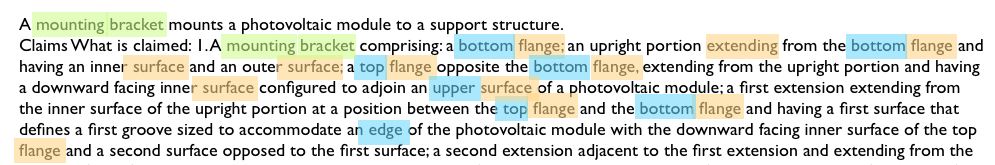
\includegraphics[width=\textwidth]{fig/pat007.png}
	\caption{A sample patent document (partial)}
	\label{sample_patent}
\end{figure}

For example, given a sample patent text, we assume that there exists a set of topics associated with this patent. In Fig.~\ref{sample_patent}, we have annotated a selection of words, with topics distinguished by colors. For the orange topic, we get words like flange, surface and extending, which could be interpreted as having something to do with attachment of hardware components such as pipes and cylinders. Similarly, the blue and green topics could be interpreted as installation and mounting respectively. By looking at the text, any human being with common comprehensive ability can easily tell what a document similar to Fig.~\ref{sample_patent} is about, and highlight the associated keywords that defines such topics. 

Nonetheless, when we scale up the size and complexity of these patent documents, using human labor to do such tasks suddenly becomes erroneous and expensive. The goal of probabilistic topic modeling is to automate this process and to provide hidden insights and meaningful intelligence of big data. If we can successfully construct a reasonable thematic structure from our patent data, we can presumably infer influences or spillovers of patent authors within the same topics.




\subsection{Latent Dirichlet Allocation}
Latent Dirichlet allocation, or LDA, is the simplest topic model \cite{lda2003} that assigns each word in the documents a distribution over a fixed number of topics. Instead of having a hard boundary between topic collections, LDA provides a distribution of topics per document, giving the likelihood of a mixed proportion of topic assignments. Namely, all patent documents share the same set of topic collection but with different proportions to each topic. For instance in Fig.~\ref{topic_proportion}, although there are $K=100$ topics overall, only a few topics were actually activated.

\begin{figure}[h]
	\center
	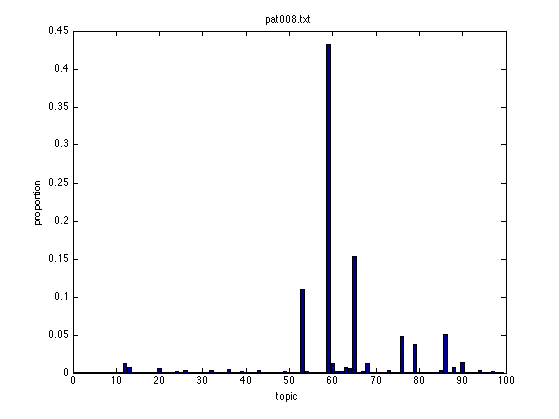
\includegraphics[width=0.55\textwidth]{fig/pat8_topics.png}
	\caption{A sample topic proportion of a patent}
	\label{topic_proportion}
\end{figure}


To build the generative probabilistic model, we compute the joint distribution and use it to estimate the posterior probability. Before jumping into the actual calculation, let's formalize our notations:

\begin{description}
	\item [$\beta_k,\; k = 1 \cdots K$]: the K topics, represented by a distribution over words
	\item [$\theta_d,\; d = 1 \cdots D$]: topic proportions for document d, where $\theta_{d,k}$ is the topic proportion of topic k for document d
	\item [$z_d,\; d = 1 \cdots D$]: topic assignments for document d, where $z_{d,n}$ is the topic assignment for the n-th word in document d
	\item [$w_d,\; d = 1 \cdots D$]: observed words for document d, where $w_{d,n}$ is the n-th word in document d
\end{description}

With the above notation, the LDA generative process can be formalized as the following joint probability of both hidden and observed random variables:

\begin{equation*}
	p(\beta_{1:K}, \theta_{1:D}, z_{1:D}, w_{1:D})\\
	= \prod_{i=1}^K p(\beta_i)\prod_{d=1}^D p(\theta_d) \left( \prod_{n=1}^N p(z_{d,n} | \theta_d) p(w_{d,n} | \beta_{1:K}, z_{d,n})\right)
\end{equation*}

which can alternatively be expressed as a graphical model:
\begin{figure}[h]
	\center
	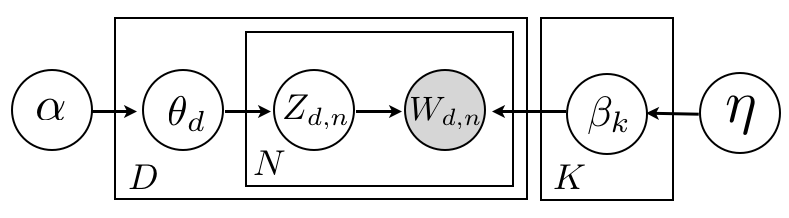
\includegraphics[width=0.75\textwidth]{fig/gm.png}
	\caption{LDA graphical model. Nodes represent variables, while edges indicate the dependency relations. The shaded node is the only observed variable (document words), and all others are the hidden variables. The $D$ plate denotes the replicated variables product over $D$ documents, while the $N$ plate denotes replication over $N$ words in each document.}
	\label{graphical_model}
\end{figure}

Note that there are several conditional dependencies implied in the graphical models, which reflects the main principles of how LDA ``think'' the documents are generated:

\begin{enumerate}
\item Randomly pick a distribution $\theta_d$ over topics.
\item For each word in the document
	\begin{enumerate}
	\item Randomly choose a topic from the previously-chosen distribution $\theta_{d,n}$.
	\item Randomly choose a word from the corresponding distribution $Z_{d,n}$.
	\end{enumerate}
\end{enumerate}

Assuming this generative process is how our documents are created, now LDA uses the graphical model in Fig.~\ref{graphical_model} to infer the posterior probability of the hidden structures given our observable:

\begin{equation*}
p(\beta_{1:K}, \theta_{1:D}, z_{1:D} | w_{1:D}) = \frac{p(\beta_{1:K}, \theta_{1:D}, z_{1:D}, w_{1:D})}{p(w_{1:D})}
\end{equation*}

The computation of possible topic structures is often intractable and the posterior distribution can only be approximated in most cases. To form an approximation algorithm, topic modeling can generally be categorized as sampling-based algorithms and variational algorithms. The most popular sampling method for topic modeling is Gibbs sampling, which introduces a sequence of random variables to construct a Markov chain and collects samples from the limiting distribution to estimate the posterior. Instead of using samples to approximate the posterior, variational methods find the closest parameterized distribution candidate by solving optimization problems \cite{lda2003} \cite{bach2010}.

\begin{figure}[h]
	\center
	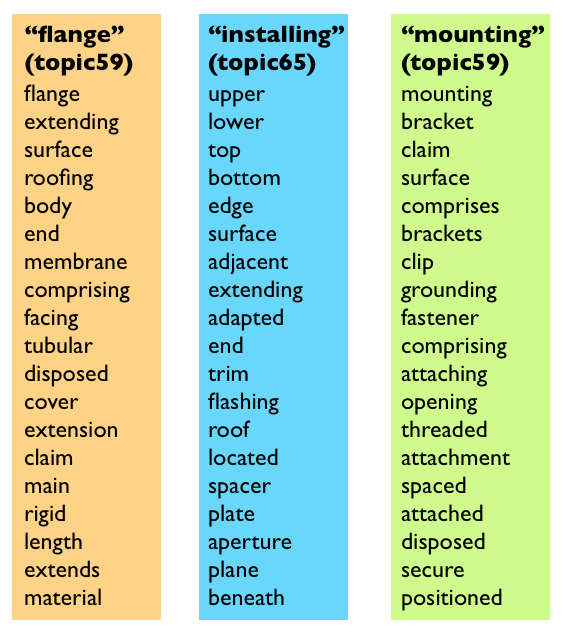
\includegraphics[width=0.5\textwidth]{fig/topics.png}
	\caption{The top 3 topics of a sample patent}
	\label{top3topics}
\end{figure}





\subsection{Limitations \& Potential Improvements}
Although LDA provides a powerful perspective to browsing and interpreting the implicit topic structures in our patent corpus, there are a few limitations it imposes against further discoveries. An extensive amount of research has been focused on relaxing some of the assumptions made by LDA to make it more flexible and suitable for various adaptations in more sophisticated context. 

\begin{description}
	\item[Bag of Words] LDA is essentially a bag-of-words probabilistic model. Namely, it constructs a word-frequency vector for each document but disregards the word ordering and the neighboring context. Although this assumption looses the syntactic information and sometimes seems unrealistic when processing natural language, it is usually good enough when capturing the document semantics and simplifying hidden structural inferences. Nonetheless, for more sophisticated tasks such as language generation or writing style modeling, the bag-of-words assumption is apparently insufficient and needs to be relaxed. In these cases, there are variants of topic models that generate topic words conditioned on the previous word \cite{wallach2006}, or switches between LDA and hidden Markov models (HMM) \cite{griffiths2005}.
	\item[Document Ordering] The LDA graphical model in Fig.~\ref{graphical_model} is invariant to the ordering of our patent documents, which could be inappropriate if the hidden thematic structure is actually dependent on sequential information such as years published, which is typical in document collections spanning years, decades or centuries. To discover how the topics change over time, the dynamic topic model \cite{blei2006} treats topics as a sequence of distributions over words and tracks how they change over time.
	\item[Fixed Number of Topics] In either LDA or more sophisticated dynamic topic models \cite{blei2006}, the number of topics $\beta_{1:K}$ is determined manually and assumed to be fixed. One elegant approach provided by the Bayesian nonparametric topic model \cite{teh2006} is to find a hierarchical tree of topics, in which new documents can now imply previously undiscovered topics.
	\item[Meta-data] To include additional attribute information associated with the documents such as authorships, titles, geolocation, citations and many others, an active branch of research has been performed to incorporate meta-data in topic models. The author-topic model \cite{rosen-zvi2004} associates author similarity based on their topic proportions, the relational topic model \cite{blei2010} assumes document links are dependent on their topic proportion distances, and more general purpose methods such as Dirichlet-multinomial regression models \cite{mimno2008} and supervised topic models \cite{blei2007}.
	\item[Others] Many other extensions of LDA are available, including the correlated topic model \cite{blei2007a}, pachinko allocation machine,  \cite{li2006}, spherical topic model \cite{reisinger2010}, sparse topic models \cite{wang2009} and bursty topic models \cite{doyle2009}.
\end{description}

\subsection{MALLET}
The Java-based package we used for topic model training is called MAchine Learning for LanguagE Toolkit (MALLET), developed by the team led by Prof. McCallum at the University of Massachusetts Amherst \cite{mallet}. It covers various algorithms for statistical natural language processing, document classification, clustering, topic modeling, information extraction and many other text-based machine learning applications, including Hidden Markov Models (HMM), Conditional Random Fields (CRF), decision trees and others. More importantly, the MALLET topic modeling toolkit provides sample-based implementations of LDA, pachinko allocation and Hierarchical LDA.

\section{Methodology}
The methodology we decided to use consists of a few carefully planned stages that put together reasonable results for patent classification and analysis of knowledge spillover patterns in the field of solar energy. As mentioned previously, we have focused primarily on applying methods of clustering in our solutions. The main tool that we used throughout the course of this project is MALLET (Machine Learning for Language Toolkit), discussed in previous sections. The main features supplied by MALLET that we took advantage of are Topic Modeling and Classification.

Very soon into the project, it became clear that the best way of tackling the problem is through clustering. The nature of knowledge spillover is such that at the beginning there is not much data given on how the knowledge is being transferred. This ruled out classification or regression methods at least in the initial stage. We decided to choose MALLET as the toolkit package that we would be working with. Written in Java and open source, it provides very good tools for textual analysis and is relatively easy in use and access. Having a wide range of features, MALLET would allow us to try different approaches and to limit the need to use other outside tools.

As mentioned before, our data source was supplied by a research group supervised by Dr Rai. The database we received was handpicked by this group, and one of our major concerns was how to handle inconsistent and incomplete entries. We ended up accessing United States Patent and Trademark Office (USPTO) website in order to obtain fuller and better representation of the data that we had initially received. After resolving our initial concerns and cleaning up our database, we could concentrate on the actual use of available resources in order to come up with a method to find out the hidden patterns and to infer knowledge spillovers.


\subsection{Feature Selection \& Construction}
First issue that we encountered and that we had to spend considerable amount of time on was data pre-processing. Cleaning up the data and deciding which parts of patent text are the most suitable to use for the task at our hands turned out to be quite tricky. Though discussion with Dr. Rai's group, we concluded that the most representative sections of patent documents  are the abstract and claims. Abstracts show the shortest and the most concise understanding of what the patent is about, and therefore seem to be suitable for our needs. Nonetheless, abstracts are usually not long enough to present a considerable value in data mining applications alone. The best choice for the supplementary field turned out to be the ``claims'' section in a patent document, as they are the essence of what an innovation has accomplished. The citations often contain redundant entries that are presented only to protect the patent from lawsuits. Similarly, description often involves the whole historical and technical background of the patent and the inventor, which are not as relevant as the abstract and claims to our objectives.

To obtain these fields, a web crawling script was created in Java that crawled USPTO�s website in order to get the required data fields. The script used patent or application numbers to access the right patent or application webpage. At this point, the abstract and claims fields were extracted from the webpage to form the final entry. The main difficulties with this step were the inconsistent markup formats and invalid patent numbers. 

\subsection{Topics Inferences}
After getting the data, the next step was to run topic modeling on the obtained patent text. The details about how topic modeling works are provided in the previous section, so in this section we will focus on how topic modeling was applied to our dataset. 

The data for each patent (i.e. the abstract and claims) is separated into individual files under a common directory. All of these files were supplied to MALLET together with a standard ``stop words'' list for English to perform the topic modeling on the data. When running topic modeling, we tried to come up with different number of topics $K$. After a few runs and result analysis, we decided to pick $K=15$ topics. Since topic modeling converges to slightly different results for each trials, we ran the algorithm multiple times to confirm that choosing $K=15$ gives us a consistent result of topics. An example of a topic model can be seen on Fig.~\ref{sample_topics}

\begin{figure}[h]
	\center
	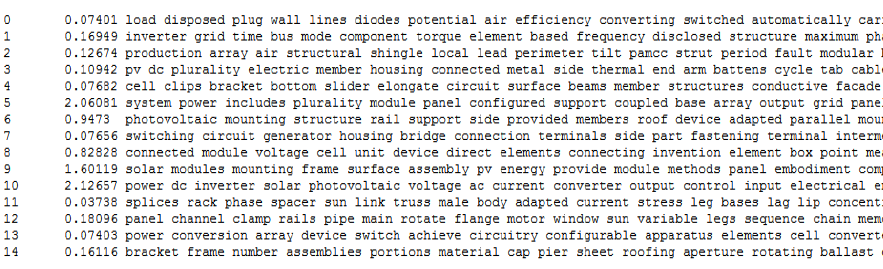
\includegraphics[width=\textwidth]{fig/sample_topics.png}
	\caption{An example of a topic model}
	\label{sample_topics}
\end{figure}


\subsection{Evaluation}
To see whether the topic models we arrived with are reasonable and reflect the actual patents distribution well, we came up with a method that would compare our results from topic models with the assigned CPC class numbers. CPC (Cooperative Patent Classification) classes are assigned by patent officers at USPTO before they are published; each patent is assigned one or more CPC classes as its application is filed to USPTO, and we use these class information to measure if our topic models constitute a valid thematic structure.


\subsection{Geographic \& Temporal Analysis}

The distribution of patents by countries can be seen on Fig.~\ref{geo_histogram} We divided geographical locations with various granularities according to their patent population. For instance, California was divided into two regions--the Bay Area and Southern California, while countries with very few samples are grouped into regions or even continents. Using the topic models we obtained in the previous steps, we can observe whether certain topics are more popular in  a selection of locations, and thus inferring relevant patterns of knowledge spillovers.

\begin{figure}[h]
	\center
	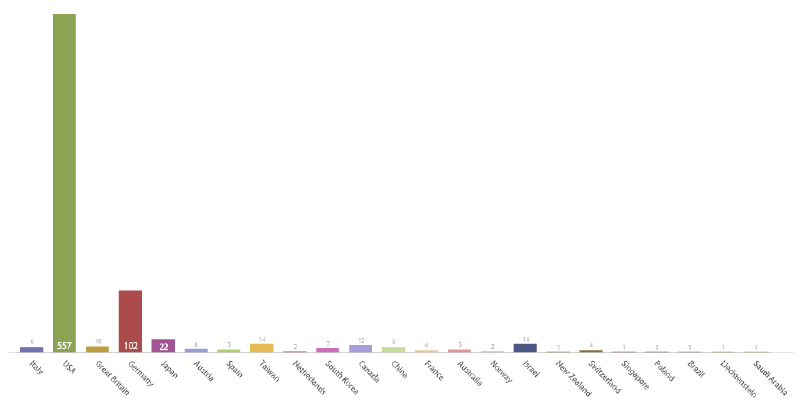
\includegraphics[width=.75\textwidth]{fig/geo_histogram.png}
	\caption{A distribution of patents by countries}
	\label{geo_histogram}
\end{figure}


Similarly, we divided patents by years and subsequently classified them into topics to observe patterns of topics trending over time. This task was more challenging in that the solar technology innovation field is relatively new, and thus the distribution over the years was rather not uniform. In Fig.~\ref{year_histogram}, we can see all patents grouped by year and the technology areaa.


\begin{figure}[h]
	\center
	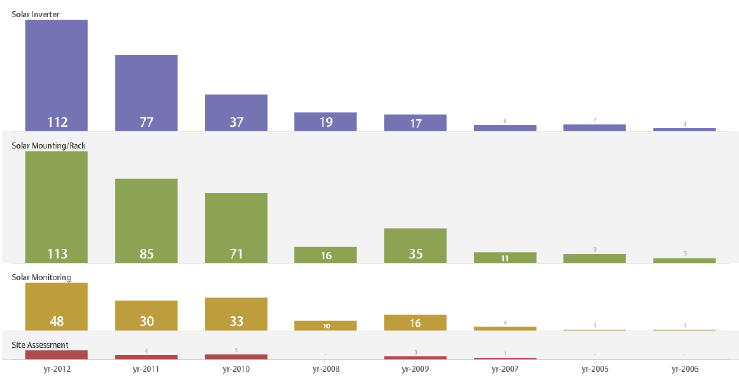
\includegraphics[width=\textwidth]{fig/year_histogram.png}
	\caption{A distribution of patents by years and technology areas}
	\label{year_histogram}
\end{figure}
Following the procedures above, we measured our topic modeling results by comparing how they are mapped by the CPC classes within the groups. This step was performed to ensure that our topic models, even when patents are divided into groups by geographies or years, still make sense and represent the actual topics that patents relate to.

Finally, the last step was to visualize the data to notice any patterns in knowledge spillover in the field of solar energy. It is much easier to see these patterns visually than in numerical and textual form. This allowed us to find any trends in the distribution of the topics and possibly to find out whether we can use data mining techniques to see whether and to what extent there is knowledge spillover in solar energy technology field. Next part of this paper will attempt to analyze the results that we have arrived with and to evaluate these results.

\section{Results}
We have run MALLET topic modeling on the solar energy patents data (claims and abstracts) carefully handpicked and crawled from the USPTO website. The objective was to determine whether data mining techniques could be used to predict and see knowledge spillover patterns in the field of solar power technology. The method we used consisted of running topic modeling on the patents then evaluating topic models by analysing whether they overlap with CPC classes to which each patent is assigned by the USPTO at the point of filing the patent application. Grouping the patents by geographies and years allowed us to see whether there appear to be any patterns in the development of patents that would imply knowledge spillover. This section of the paper is presenting the results that we have obtained.

The first question that is crucial to any further consideration of the results is whether we can use topic modeling to classify patents in the first place. This could be evaluated by computing whether patent topics obtained through topic modeling overlap with either technology area or/and CPC classes. There are 4 broad technology areas that patents cover: Solar Monitoring, Solar Mounting/Rack, Solar Inverter and Site Assessments. There are 23 CPC classes that patents composing our data represented. The overlap between the true class and modelled class obtained for topic modeling is presented in Table~\ref{results_table}. Fig.~\ref{ta_results_matrix} is a graphic representation of the confusion matrix of patents� classification using topic modeling and technology areas.

\-\\
\begin{table}
\centering
\begin{tabular}{|l|l|}
\hline
Coarse-grained (technology area) & Fine-grained (CPC Class)\\
\hline
79.49\% & 81.01\% \\
Exact match & Match 1-out-of-3 predicted to top 3\\
\hline
\end{tabular}
\caption{Results}
\label{results_table}
\end{table}



\begin{figure}[h]
	\center
	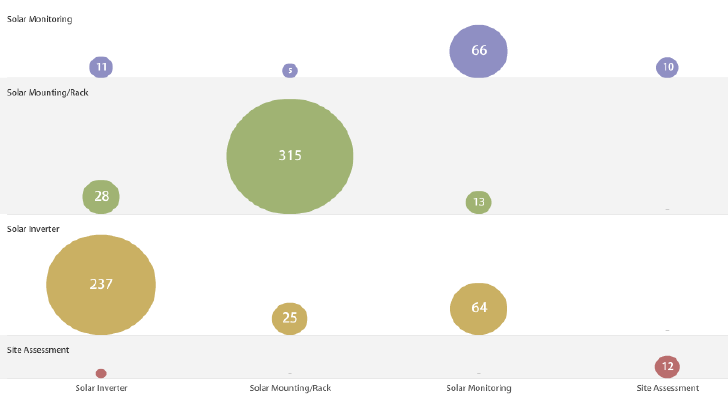
\includegraphics[width=0.75\textwidth]{fig/ta_results_matrix.png}
	\caption{The confusion matrix of our predicted technology area results.}
	\label{ta_results_matrix}
\end{figure}


The above data suggests that the classification of patents based on topic modeling is good and we can say with a significant degree of confidence that topic modeling can be used for the purpose of patent classification.

Next step is evaluating whether patents are associated with specific geographies and can topic modeling predict these associations. To answer these questions patents were divided into geographies and then classification based on topic models was performed on the patents. In Fig.~\ref{original_ta_geo} and Fig.~\ref{our_ta_geo} respectively we can see the most popular actual technology area and the most popular predicted technology area using topic modeling. Both seem to overlap almost completely and therefore, we can confidently give a positive answer to this problem.

\begin{figure}[ht]
%	\center
	\begin{minipage}[b]{0.5\linewidth}
		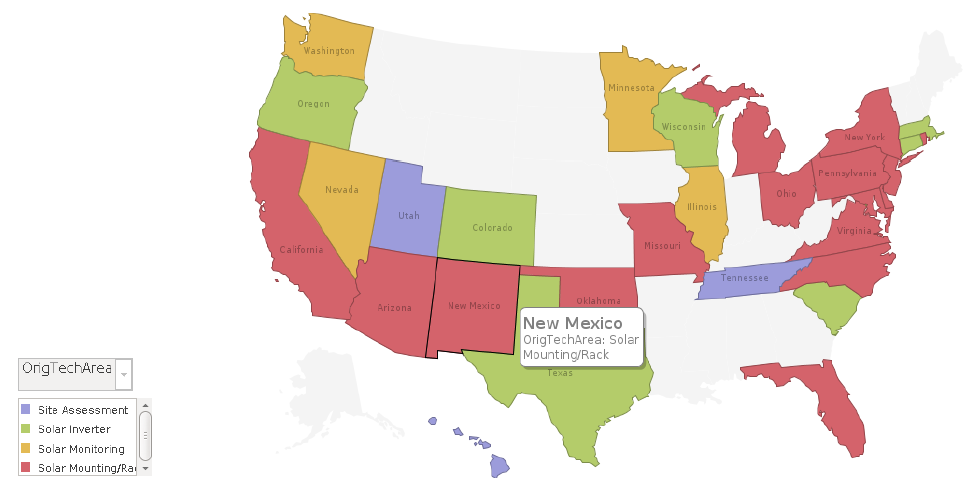
\includegraphics[width=\textwidth]{fig/original_ta_geo}
		\caption{The original technology area distributed over geolocation}
		\label{original_ta_geo}
	\end{minipage}
	\hspace{0.5cm}
	\begin{minipage}[b]{0.5\linewidth}
		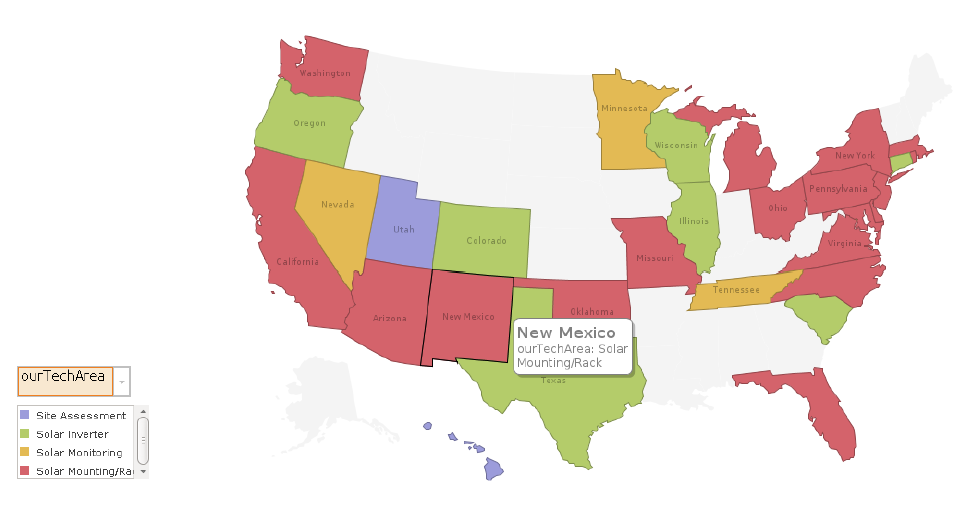
\includegraphics[width=\textwidth]{fig/our_ta_geo}
		\caption{Our predicted technology area distributed over geolocation}
		\label{our_ta_geo}
	\end{minipage}
\end{figure}

As we observed above there are patents associated with specific geographies and topic modeling can identify that quite accurately. This result assures us that topic modeling is a valid method of classifying patents.

However, the real question that we are interested in for the purpose of this paper is whether we can detect knowledge spillovers in the field of solar energy using data mining techniques. For this part we have focused mostly on the data pertaining to the United States, since there is simply not enough data from other countries and if there is then there is not enough granularity in the geographical location data. To answer the question of detecting knowledge spillovers, it will be very helpful to visualize the results in the form of a US map that is color-coded by different topics that are the most popular in each state. This graph can be seen in the Fig.~\ref{topics_geo}

\begin{figure}[h]
	\center
	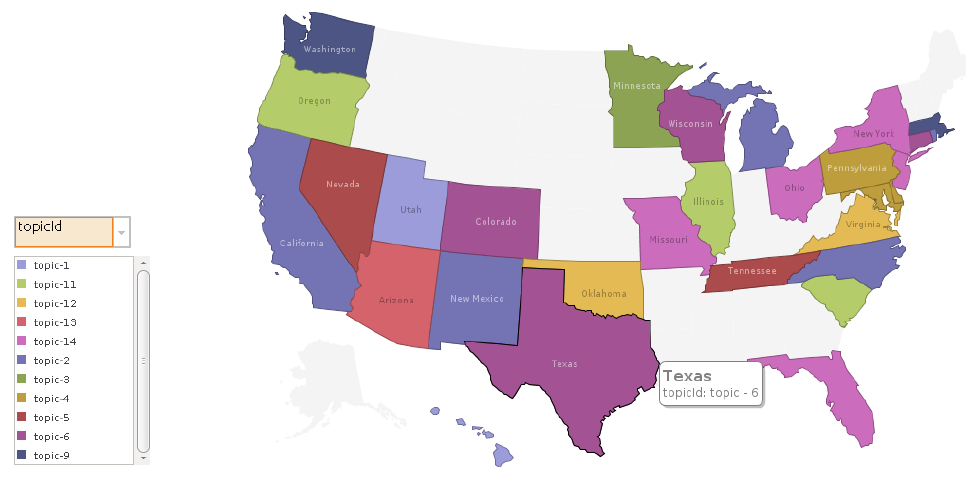
\includegraphics[width=0.5\textwidth]{fig/topics_geo.png}
	\caption{The most popular topics in each state of the U.S.}
	\label{topics_geo}
\end{figure}

Each color in Fig.~\ref{topics_geo} represents the topic that is the most popular in each state. We can see that on the graph above topics themselves are not directly very meaningful when it comes to geographical distribution of the patents. The colors in general are distributed all over the place. However, we can see that purple-pink color is more popular in the South and East while blue is more popular in the West and green in the North. These assumptions are, however very weak and based on subjective heuristic perceptions. In overall, although we can see some patterns forming to some degree, we cannot see a clear pattern of knowledge spillover that would clearly support any thesis on knowledge spillover in solar energy field. Therefore, we concluded that although it looks like it would be possible to use topic modeling to mine for knowledge spillovers, we are not yet there and some further iterations and more complex models would need to be applied in order to obtain an acceptably meaningful and refined solution.

Another question that we are trying to find an answer to is whether we can mine for knowledge spillover across different years. This is whether there are any topics that become especially popular after given years or in given time periods. We can see the distribution of topics among years in Fig.~\ref{topics_year}



\begin{figure}[h]
	\center
	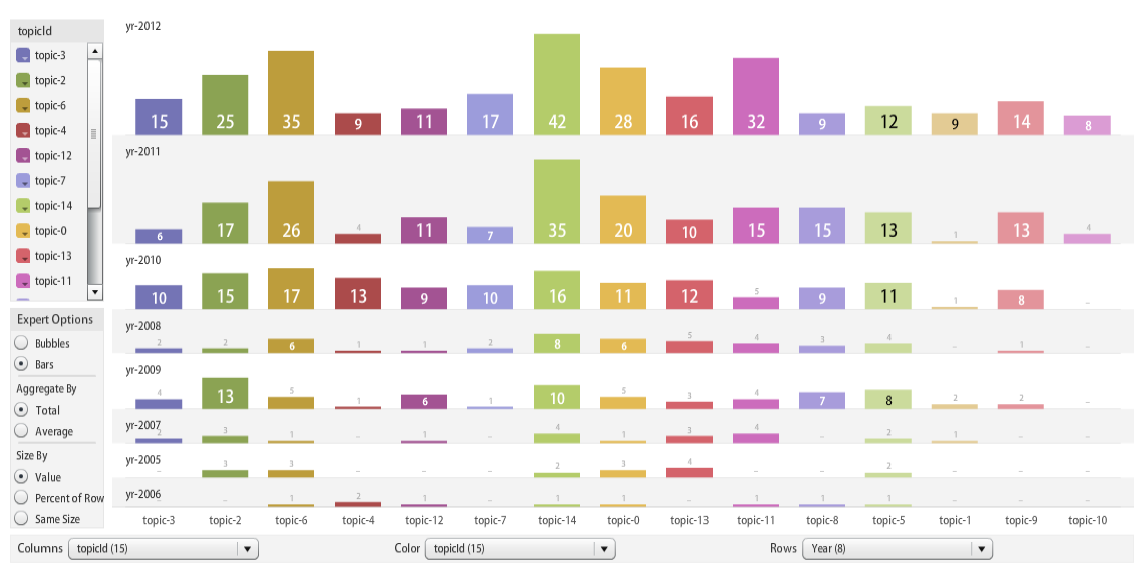
\includegraphics[width=0.75\textwidth]{fig/topics_year.png}
	\caption{The topics population over years}
	\label{topics_year}
\end{figure}
On the graph it can be clearly seen that the distribution of topics does not change much from year to year. It basically stays the same throughout the whole period under consideration in this paper. It should be noted that the overall number of patents in solar energy field is growing from year to year and this is most likely caused by more incentives to move towards renewable energy sources coupled with rising prices of conventional energy sources. However, there seems to be no possibility of measuring knowledge spillover across the years using topic modeling methods, apart from the fact that there is similar distribution of topics from year to year and establishing what this distribution is.

\section{Conclusion}



The project�s objective was to analyze around 800 patents from solar energy field and come up with data mining techniques that could help with knowledge spillover analysis and prediction in this field. We have crawled the data from USPTO website, using for the purpose of this project fields of abstract and claims in the text of patents. After this step, we clustered patents based on topics that they correspond to. We evaluated the topics by checking whether based on information about topics the original classification of patents can be obtained. Finally, we visualized and interpreted the results with respect to patent CPC classes (classes assigned by patent officers at USPTO), geographical distribution and time i.e. when patent has been invented. The analysis of the results allowed us to come up with answers to the vital questions pertaining the issue at hand.

The analysis of the results gives an idea of whether the knowledge spillover can be measured using topic modeling methods. We have used MALLET (Machine Learning for Language Toolkit) to perform topic modeling and classification based on topic models tasks. The data that we used this is claims and abstracts of patents and applications for patents from solar energy fields from years 2006-2012 show that Topic Modeling is a viable method of patents classification. Using Topic Modeling gives rate of success on the data we had crawled from USPTO website of up to 81\%. This is a good rate of success suggesting that most of the patents are classified correctly.

As for geographical distribution, we can see that there are interesting patterns in the geographical distribution of patents that can be noted. These patterns can be detected using topic modeling at least to some extent. We showed that it is possible to show which technology is the most popular in each area based on topic modeling and that this data overlaps with the actual technology areas popular in these regions. Furthermore, we can see that some very weak patterns are being formed even at the level of single topic models (not assembled into technology area groups). These features of topic models can be of significant use when analyzing temporal changes in the field of solar energy. Similarly, they can be of use when trying to figure out local interests in research in the field. And so we know that Texas for example is more interested in research into Solar Inverters and California is more focused on Solar Mounting and Racks.

As for the temporal analysis of patents there has not been much data that would support the thesis that topic modeling could be used to predict and notice patterns in knowledge spillover. The distribution of topics across different years has not been changing much. The only reasonable conclusion that we can draw from the data under consideration is the fact that number of patents in the solar energy fields is growing but this is not a surprising fact as alternative energy sources are becoming more and more popular in recent years. Also, there is no great range on the time scale in the field of solar energy as this is a very new field. 

Therefore, the temporal analysis could be performed only on the period of 6 years and this could affect the outcome of our results. Analyzing more established field could lead to more meaningful conclusion in terms of how knowledge spillovers can be measured using topic modeling of patents. Furthermore, the data was mostly handpicked, which means that there is a possibility that some entries were discarded or added to the data set based on subjective opinions or simply because of human error. This could also impact our results.

The hardest tasks that we had to deal with throughout the course of this project were: data pre-processing, inferences and visualizing the data to confirm the hypotheses. Data pre-processing including crawling the data from the USPTO website and sorting out the right Application and Patent numbers took us significant time and effort. Also visualizing the data to show the results in the nice fashion using clear and understandable graphics was not a very easy task. The color-coded maps where a real challenge to master and develop.


\section{Future Works}
Due to the time constraints we were unable to address all possible solutions and to approach the problem from every possible angle. There is still plenty of room left for improvements and further extensions to the procedures we performed. Similarly, there are few other approaches that we could have tried in order to receive even more satisfying solutions.
One obvious approach that we could use and adapt to our solution in order to refine our topic modeling is the use of Natural Language Processing (NLP) and phrases analysis. This would mean mining for the topics based on phrases and pairs of words rather than single words alone. Such a development would hopefully lead to more accurate topic models and in turn better classification method.

Another possible modification to our topic modeling would be to utilize a supervised topic modeling algorithm. These algorithms, such as the supervised latent Dirichlet allocation algorithm (sLDA) \cite{blei2007} allow users to manually influence their topic modeling. This serves the purpose of modeling text more accurately for a specific purpose. For example, a standard topic model of the text of an entire patent may return several topics specific to patents but not the text area (such as the terms �figure� or �table). Through the use of a supervised method, the user can guide the topics towards terms such more specific to their goals. In our case these would be terms relevant to solar technologies.

Furthermore, a good idea to research would be attempting and testing the method with patents from different areas. This would allow us to see whether the algorithm is applicable to different technology areas and check the universality of the algorithm. Extending the project for possibly patents from any area would be a great research opportunity that would take a significant amount of time but could produce very interesting results.

Defining a more adequate stop words definition is an aspect of our method that we could further work on. This would hopefully improve our topic modeling classification method since words that are specific to all patents would be omitted while constructing the topic models. We were initially going to attempt this s improvement, however, it turned out that regular stop words list for English language delivered satisfying results so we left this as an option towards the end of our time schedule and we simply did not have time at the end. Nevertheless, it would be an interesting opportunity to work on a development of patent specific stop words list.

Another factor that could contribute to spillovers and possibly mining in it could give us some insight on knowledge transfer is size and type of the owner of a patent assignee i.e. the entity that owns the patent. Therefore, researching the distribution of patents based on the type and size of their assignees was suggested to us as another factor that we could consider in our project. Definitely work on it could lead to some meaningful insights on knowledge spillover.

Lastly, we could use a data set that represented patents more uniformly distributed in time and over wider domain (more than 6 years). This could be achieved at least in theory by the use of stratified sampling. Having wider domain and more uniformly distributed patents could lead to a better conclusions regarding the knowledge spillover in time. However, we have to keep in mind that this may not be possible at all in the first place as the solar energy field is very new field and there is not many patents available that were granted or filed before 2005. Attempting a different, more established, field and a wider time domain could be a good substitute for this further development.


\section{Acknowledgements}


\begin{thebibliography}{1}

\bibitem{us_patent}
The United States Patent and Trademark Office, http://www.uspto.gov/patents/process/search/. 2012
\bibitem{mallet}
McCallum, Andrew Kachites.  "MALLET: A Machine Learning for Language Toolkit."
    http://mallet.cs.umass.edu. 2002.
\bibitem{TLY07}
Yuen-Hsien Tseng, Chi-Jen Lin, Yu-I Lin. Text mining techniques for patent analysis. Information Processing and Management, Volume 43, Issue 5, September 2007. http://www.sciencedirect.com/science/article/pii/S0306457306002020
\bibitem{TLY03}
Tao Liu, Shengping Liu, Zheng Chen, and Wei Y. Ma. �An evaluation on feature selection for text clustering. 
	Proc. 20th International Conference on Machine Learning (ICML03), August 2003.
\bibitem{MM10}
Martin Moehrle. Measures for textual patent similarities: a guided way to select appropriate approaches. Scientometrics, May 2010. 
	http://link.springer.com/article/10.1007\%2Fs11192-010-0243-3?LI=true\#
\bibitem{geography}
Peter Thompson. Patent Citations and the Geography of Knowledge Spillovers: Evidence from Inventor- and Examiner-added Citations The Review of Economics and Statistics. 2006

\bibitem{blei2011}
Blei, D. Introduction to Probabilistic Topic Models. Princeton University. 2011.

\bibitem{lda2003}
Blei, D., Ng, A. and Jordan, M. Latent Dirichlet allocation. Journal of Machine Learning Research, 3:993-1022, January 2003.

\bibitem{bach2010}
Hoffman, M., Blei, D. and Bach, F. On-line learning for latent Dirichlet allocation. In Neural Information Processing Systems, 2010.

\bibitem{wallach2006}
Wallach, H. Topic modeling: Beyond bag of words. In Proceedings of the 23rd International Conference on Machine Learning, 2006.

\bibitem{griffiths2005}
Griffiths, T., Steyvers, M., Blei, D. and Tenenbaum, J. Integrating topics and syntax. In L. K. Saul, Y. Weiss, and L. Bottou, editors, Advances in Neural Information Processing Systems 17, pages 537-544, Cambridge, MA, 2005. MIT Press.

\bibitem{blei2006}
Blei, D. and Lafferty, J. Dynamic topic models. In International Conference on Machine Learning, pages 113-120, New York, NY, USA, 2006. ACM

\bibitem{teh2006}
Teh, Y., Jordan, M., Beal, M. and Blei, D. Hierarchical Dirichlet process. Journal of the American Statistical Association, 101(476):1566-1581, 2006.

\bibitem{rosen-zvi2004}
Rosen-Zvi, M., Griffiths, T., Steyvers, M. and Smith, P. The author-topic model for authors and documents. In Proceedings of the 20th Conference on Uncertainty in Artificial Intelligence, pages 487-494. AUAI Press, 2004.

\bibitem{blei2010}
Chang, J. and Blei, D. Hierarchical relational models for document networks. Annals of APplied Statistics, 4(1), 2010.

\bibitem{mimno2008}
Mimno, D. and McCallum, A. Topic models conditioned on arbitrary features with Dirichlet-multinomial regression. In Uncertainty in Artificial Intelligence, 2008.

\bibitem{blei2007}
Blei, D. and McAuliffe, J. Supervised topic models. In Neural Information Processing Systems, 2007.

\bibitem{blei2007a}
Blei, D. and Lafferty, J. A correlated topic model of Science. Annals of Applied Statistics, 1(1):17-35, 2007.

\bibitem{li2006}
Li, W. and McCallum, A. Pachinko allocation: DAG-structured mixture models of topic correlations. In International Conference on Machine Learning, pages 577-584, 2006.

\bibitem{reisinger2010}
Reisinger, J., Waters, A. ,Silverthorn, B. and Mooney, R. Spherical topic models. In International Conference on Machine Learning, 2010.

\bibitem{wang2009}
Wang, C. and Blei, D. Decoupling sparsity and smoothness in the discrete hierarchical dirichlet process. In Y. Bengio, D. Schuurmans, J. Lafferty, C. K. I. Williams, and A. Culotta, editors, Advances in Neural Information Processing Systems 22, pages 1982-1989. 2009.

\bibitem{doyle2009}
Doyle, G. and Elkan, C. Accounting for burstiness in topic models. In International Conference on Machine Learning, pages 281-288. ACM, 2009.

\end{thebibliography}
%

\end{document}  
